\documentclass[10pt,a4paper]{article}
\usepackage[margin=2.2cm]{geometry}
\usepackage{newtxtext,newtxmath}
\usepackage{graphicx,booktabs,amsmath,xcolor,float,caption}
\usepackage[hidelinks]{hyperref}
\captionsetup{font=small,labelfont=bf}
\graphicspath{{figures/}}
% generated by scripts/gate_bump_study.py
\newcommand{\BmpSeventyFive}{0.99}
\newcommand{\BmpSixty}{0.98}
\newcommand{\BmpFortyEight}{0.96}
\newcommand{\BmpDivider}{1.06}
\newcommand{\BmpNegOneSF}{-0.01}
\newcommand{\BmpNegTwoSF}{-1.01}
\newcommand{\BmpCOneSF}{0.82}
\newcommand{\BmpCTwoSF}{0.68}
\newcommand{\BmpNegOneCOneSF}{-0.18}
\newcommand{\BmpNegOneSix}{-0.02}
\newcommand{\BmpNegTwoSix}{-1.02}
\newcommand{\BmpCTwoSix}{0.67}
\newcommand{\VgsMinNegTwo}{-3.26}
\newcommand{\VgsLMinNegTwo}{-3.09}
\newcommand{\OvsSF}{11.5}
\newcommand{\OvsSix}{10.7}
\newcommand{\OvsFE}{11.6}
\newcommand{\VmEighty}{57}
\newcommand{\VmNinety}{66}
\newcommand{\VmEightyK}{69}
\newcommand{\VmNinetyK}{79}
\newcommand{\VpkSF}{101}
\newcommand{\VpkSix}{83}
\newcommand{\EtaSF}{99.53}
\newcommand{\EtaSix}{99.44}
\newcommand{\EtaFE}{99.32}
\newcommand{\EtaSFNegTwo}{99.52}
\newcommand{\EtaSixNegTwo}{99.43}
\newcommand{\EtaSFCTwo}{99.52}
\newcommand{\PswSix}{1.41}
\newcommand{\PswFE}{1.04}
\newcommand{\PdeadNegTwo}{0.38}
\newcommand{\PgateNegTwo}{0.05}
\newcommand{\PgateCTwo}{0.04}
\newcommand{\EonSF}{40.9}
\newcommand{\EonSix}{29.9}
\newcommand{\EoffSF}{8.0}
\newcommand{\EonSFCTwo}{49.6}
\newcommand{\EoffSFCTwo}{7.9}
\newcommand{\EonSFNegTwo}{42.8}
\newcommand{\EoffSFNegTwo}{7.8}
\newcommand{\DvOnSF}{13}
\newcommand{\DvOnSix}{7}
\newcommand{\InvLossSF}{704}
\newcommand{\NsmSF}{16}
\newcommand{\NtrSF}{192}
\newcommand{\NdrvSF}{48}
\newcommand{\PtrSF}{762}
\newcommand{\VpkSFk}{101}
\newcommand{\VpkSFone}{86}
\newcommand{\UtilSF}{75}
\newcommand{\InvLossSix}{845}
\newcommand{\NsmSix}{20}
\newcommand{\NtrSix}{240}
\newcommand{\NdrvSix}{60}
\newcommand{\PtrSix}{610}
\newcommand{\VpkSixk}{83}
\newcommand{\VpkSixone}{71}
\newcommand{\UtilSix}{60}
\newcommand{\InvLossFE}{1023}
\newcommand{\NsmFE}{25}
\newcommand{\NtrFE}{300}
\newcommand{\NdrvFE}{75}
\newcommand{\PtrFE}{488}
\newcommand{\VpkFEk}{69}
\newcommand{\VpkFEone}{59}
\newcommand{\UtilFE}{48}

\newcommand{\BumpRows}{%
75 & 0\,V, -- & 0.99 & -1.27 & 40.9 & 8.0 & 1.91 & 0.20 & 0.03 & 99.53 \\
75 & $-1$\,V, -- & -0.01 & -2.26 & 41.8 & 7.8 & 1.94 & 0.29 & 0.04 & 99.53 \\
75 & $-2$\,V, -- & -1.01 & -3.26 & 42.8 & 7.8 & 1.98 & 0.38 & 0.05 & 99.52 \\
75 & 0\,V, 1\,nF & 0.82 & -0.97 & 45.2 & 7.9 & 2.08 & 0.20 & 0.03 & 99.53 \\
75 & 0\,V, 2\,nF & 0.68 & -0.79 & 49.6 & 7.9 & 2.25 & 0.20 & 0.04 & 99.52 \\
75 & $-1$\,V, 1\,nF & -0.18 & -1.97 & 46.3 & 7.7 & 2.11 & 0.29 & 0.05 & 99.52 \\
\midrule
60 & 0\,V, -- & 0.98 & -1.25 & 29.9 & 6.1 & 1.41 & 0.20 & 0.03 & 99.44 \\
60 & $-1$\,V, -- & -0.02 & -2.25 & 30.8 & 5.8 & 1.43 & 0.29 & 0.04 & 99.43 \\
60 & $-2$\,V, -- & -1.02 & -3.25 & 31.6 & 5.8 & 1.46 & 0.38 & 0.05 & 99.43 \\
60 & 0\,V, 1\,nF & 0.81 & -0.95 & 33.4 & 6.0 & 1.54 & 0.20 & 0.03 & 99.43 \\
60 & 0\,V, 2\,nF & 0.67 & -0.77 & 36.9 & 6.0 & 1.67 & 0.20 & 0.04 & 99.43 \\
60 & $-1$\,V, 1\,nF & -0.19 & -1.95 & 34.3 & 5.8 & 1.56 & 0.29 & 0.05 & 99.43 \\
\midrule
48 & 0\,V, -- & 0.96 & -1.22 & 21.9 & 4.7 & 1.04 & 0.20 & 0.03 & 99.32 \\
48 & $-1$\,V, -- & -0.03 & -2.23 & 22.6 & 4.4 & 1.06 & 0.29 & 0.04 & 99.32 \\
48 & $-2$\,V, -- & -1.03 & -3.23 & 23.3 & 4.4 & 1.08 & 0.38 & 0.05 & 99.31 \\
48 & 0\,V, 1\,nF & 0.80 & -0.93 & 24.5 & 4.6 & 1.14 & 0.20 & 0.03 & 99.32 \\
48 & 0\,V, 2\,nF & 0.66 & -0.75 & 27.3 & 4.6 & 1.25 & 0.20 & 0.04 & 99.31 \\
48 & $-1$\,V, 1\,nF & -0.20 & -1.93 & 25.3 & 4.4 & 1.16 & 0.29 & 0.05 & 99.31 \\
}

\newcommand{\uF}{\ensuremath{\mu}F}
\definecolor{box}{rgb}{0.93,0.95,0.98}

\title{\textbf{High-Side Gate Bump and Voltage Utilization\\of the EPC2361 SPB Building Block}}
\author{Enes Ayaz, KTH --- design note, simulation only}
\date{8 October 2026}

\begin{document}
\maketitle

\noindent\colorbox{box}{\parbox{\dimexpr\linewidth-2\fboxsep}{\small
\textbf{Summary.}
\begin{itemize}\itemsep0pt
\item When the low side turns on, the gate of the held-off high side rises to \BmpSeventyFive\,V (LTspice, Q3D parasitics, 75\,V, 141\,A), above the 0.8\,V minimum threshold of EPC2361.
\item The bump is the Miller charge of the high side divided onto its gate--source capacitance, $\Delta v_\mathrm{GS}\approx Q_\mathrm{GD}/C_\mathrm{GS}\approx\BmpDivider$\,V. It is almost independent of the load current (0.95--0.99\,V from 10 to 157\,A) and of the bus voltage (\BmpFortyEight, \BmpSixty{} and \BmpSeventyFive\,V at 48, 60 and 75\,V). \textbf{Neither lowering the current nor lowering the submodule voltage removes it.}
\item The bump lasts about 2\,ns above 0.8\,V. Even with the high-side threshold lowered to 0.6\,V, the simulation shows no channel shoot-through: the high-side charge (output capacitance) and $E_\mathrm{on}$ are unchanged.
\item The EPC90156 evaluation board (same transistor) uses 1\,$\Omega$/0.47\,$\Omega$ gate resistors, 0\,V off-state and no gate capacitor, and is rated for 80\,V; it has the same bump mechanism.
\item Robust fix: an off-state bias of $-1$\,V moves the peak to \BmpNegOneSF\,V (0.8\,V margin) at a cost of 0.01\,\% efficiency. $-2$\,V brings the undershoot to \VgsMinNegTwo\,V, close to the $-4$\,V limit. A 2\,nF external $C_\mathrm{GS}$ only reaches \BmpCTwoSF\,V and costs 21\,\% more $E_\mathrm{on}$.
\item Voltage utilization: with an overshoot of about 11\,V and a battery range of $k=V_{m,\max}/V_m=1.2$, the peak $v_\mathrm{DS}$ is \VpkSFk\,V for $V_m$\,=\,75\,V (above the rating) and \VpkSixk\,V for 60\,V. Keeping the peak below 80\,V (80\,\% of the rating, as EPC rates its own board) allows $V_m\le\VmEighty$\,V for $k$\,=\,1.2 and $\le\VmEightyK$\,V for a regulated bus. \textbf{The voltage limit, not the gate bump, is the reason to reduce the submodule voltage to about 60\,V} ($N$\,=\,20), at the cost of 0.09\,\% efficiency and 25\,\% more transistors.
\end{itemize}}}

\section{Observation}
In the double-pulse simulation of the building block (two EPC2361 per switch, centre driver, Q3D power loop and gate star, external $R_\mathrm{g,on}/R_\mathrm{g,off}$\,=\,2/0\,$\Omega$), the gate of the high side, which is held off through the driver pull-down, rises to about 1\,V when the low side turns on (Fig.~\ref{fig:mech}a). The datasheet threshold of EPC2361 is 0.8\,V minimum, 1.1\,V typical and 2.5\,V maximum at 25\,$^\circ$C, and it decreases with temperature (datasheet Fig.~10). A bump of this size therefore has no guaranteed margin.

\section{Mechanism}
During the low-side turn-on the high-side drain--source voltage rises from about $-2$\,V (reverse conduction) to the bus voltage within 4--6\,ns. The displacement current through $C_\mathrm{GD}$ charges the high-side gate. If the hold-off path could remove this charge instantly, the gate would stay at the off level; it cannot, because its time constants are of the same order as the transition:
\begin{equation}
\tau_{RC}=R_{G,\mathrm{off}}\,C_\mathrm{iss}\approx0.8\,\Omega\cdot3.6\,\mathrm{nF}\approx2.9\,\mathrm{ns},\qquad
\tau_{L}=L_G/R_{G,\mathrm{off}}\approx1.7\,\mathrm{nH}/0.8\,\Omega\approx2.1\,\mathrm{ns}.
\end{equation}
In the limit of a hold-off path that does not react, the Miller charge is shared between $C_\mathrm{GD}$ and $C_\mathrm{GS}$:
\begin{equation}
\Delta v_\mathrm{GS}\approx\frac{Q_\mathrm{GD}}{C_\mathrm{GS}+C_\mathrm{ext}}=\frac{3.8\,\mathrm{nC}}{3.59\,\mathrm{nF}}\approx\BmpDivider\,\mathrm{V},
\label{eq:div}
\end{equation}
and the simulated peak of 0.99\,V is close to this limit. Two consequences follow, both confirmed by the simulations (Fig.~\ref{fig:mech}b, c):
\begin{itemize}
\item \textbf{Current independence.} $Q_\mathrm{GD}$ is a property of the voltage swing, not of the current. Over 10--157\,A the peak changes by less than 0.05\,V for every gate-resistor pair, although the turn-on $dv/dt$ falls from 18 to 12\,V/ns.
\item \textbf{Weak voltage dependence.} $C_\mathrm{GD}$ of a GaN HEMT is large only at low $v_\mathrm{DS}$ and drops by orders of magnitude within the first 10--20\,V, so most of $Q_\mathrm{GD}$ is transferred early in the transition. Switching 48, 60 or 75\,V moves almost the same Miller charge: \BmpFortyEight, \BmpSixty{} and \BmpSeventyFive\,V.
\end{itemize}
A larger turn-off resistance makes the bump worse (1.10, 1.21 and 1.29\,V for 2, 5 and 10\,$\Omega$), and a slower turn-on helps little (0.94\,V for $R_\mathrm{g,on}$\,=\,10\,$\Omega$, at 2.5 times $E_\mathrm{on}$).

\begin{figure}[t]
\centering
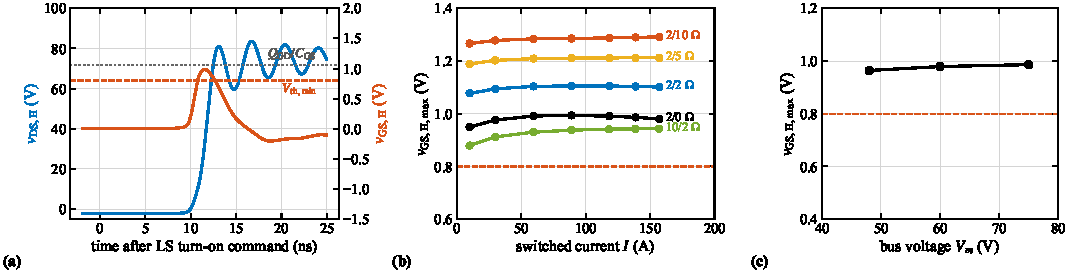
\includegraphics[width=\textwidth]{bump_mechanism.pdf}
\caption{(a) High-side drain--source and gate--source voltage during the low-side turn-on (75\,V, 141\,A, 2/0\,$\Omega$); dashed: $V_\mathrm{th,min}$, dotted: $Q_\mathrm{GD}/C_\mathrm{GS}$. (b) Peak high-side gate voltage against the switched current for five gate-resistor pairs $R_\mathrm{g,on}/R_\mathrm{g,off}$. (c) Peak high-side gate voltage against the bus voltage (141\,A, 2/0\,$\Omega$).}
\label{fig:mech}
\end{figure}

\section{Does the high side turn on?}
The bump lasts 1.5--1.9\,ns above 0.8\,V and about 3\,ns above 0.5\,V. To test whether it causes conduction, the threshold of both high-side transistors was lowered by 0.3\,V (to the datasheet minimum of 0.8\,V) and by 0.5\,V (0.6\,V) with a series voltage in the model. Table~\ref{tab:st} shows that the positive high-side charge during the low-side turn-on, which is the charging of its output capacitance, and $E_\mathrm{on}$ do not increase: the channel does not conduct measurably within the 2\,ns. In the model, the bump is therefore not harmful. The margin is nevertheless small for hardware, because the model excludes the package inductance and routing details, the threshold falls at high temperature, and the gate ringing in hardware is usually stronger than simulated. The peak itself is a narrow spike; it varies between 0.99 and 1.09\,V with the solver time step.

\begin{table}[h]
\centering\small
\caption{High-side conduction check (75\,V, 141\,A, 2/0\,$\Omega$, 0\,V off-state)}
\label{tab:st}
\begin{tabular}{@{}lccc@{}}
\toprule
High-side threshold & 1.1\,V (typical) & 0.8\,V (min.) & 0.6\,V \\
\midrule
Positive high-side charge (left die) & 221\,nC & 219\,nC & 218\,nC \\
$E_\mathrm{on}$ of the low side & 40.9\,\textmu J & 40.6\,\textmu J & 40.5\,\textmu J \\
\bottomrule
\end{tabular}
\end{table}

\section{Comparison with the EPC90156 evaluation board}
EPC's half-bridge board for the same transistor (quick-start guide and schematic Rev.\,4.0, in \texttt{Datasheet/}) does not use any special measure against the bump (Table~\ref{tab:epc}). It drives one transistor per switch with split outputs, 1\,$\Omega$ for turn-on and 0.47\,$\Omega$ for turn-off, a 0/5\,V gate drive without negative bias and without a gate--source capacitor. Its input is rated for 80\,V, i.e., 80\,\% of the transistor rating, and all measurements in the guide are at 48\,V. Since the bump is set by the device ratio $Q_\mathrm{GD}/C_\mathrm{GS}$, the evaluation board has the same order of bump; EPC accepts it, relying on the short duration shown above. What differs is the voltage derating.

\begin{table}[h]
\centering\small
\caption{Gate drive of the EPC90156 and of the building block}
\label{tab:epc}
\begin{tabular}{@{}lll@{}}
\toprule
 & EPC90156 & building block \\
\midrule
Transistors per switch & 1\,$\times$\,EPC2361 & 2\,$\times$\,EPC2361 \\
Driver & uP1966E, split outputs, 5\,V & LT8418, split outputs, 5\,V \\
$R_\mathrm{g,on}$ / $R_\mathrm{g,off}$ (external) & 1 / 0.47\,$\Omega$ & 2 / 0\,$\Omega$ \\
Off-state bias / $C_\mathrm{GS,ext}$ & 0\,V / none & 0\,V / none \\
Hold-off path & one pull-down per transistor & one pull-down shared by two, star with $L_G$\,=\,1.71\,nH \\
Rated input voltage & 80\,V (measured at 48\,V) & 75\,V nominal \\
Rated current & 40\,A & 100\,A$_\mathrm{rms}$ (141\,A peak) \\
\bottomrule
\end{tabular}
\end{table}

\section{Mitigation}
The model was extended by an off-state bias $-V_\mathrm{neg}$ of the driver (both drivers) and an external capacitor $C_\mathrm{ext}$ from every gate pad to its source pad, and simulated for $V_\mathrm{neg}$\,=\,0, 1, 2\,V, $C_\mathrm{ext}$\,=\,0, 1, 2\,nF and 48, 60, 75\,V (\texttt{simulation/bb\_spice/BB\_bump.cir}, 27 cases). The leg loss uses the switching energies of each case, the dead-time loss with the reverse-conduction drop increased by $V_\mathrm{neg}$, and the gate-drive loss including $C_\mathrm{ext}$ (Fig.~\ref{fig:mit}, Table~\ref{tab:mit}).
\begin{itemize}
\item \textbf{Negative off-state bias} shifts the whole waveform: the peak follows $-V_\mathrm{neg}$ almost exactly (\BmpNegOneSF\,V for $-1$\,V, \BmpNegTwoSF\,V for $-2$\,V at 75\,V). The cost is small: the dead-time loss rises from 0.20 to \PdeadNegTwo\,W at $-2$\,V and the turn-off becomes slightly faster, which raises the low-side overshoot from 86.5 to 90.2\,V at $-2$\,V. At $-2$\,V the high-side gate undershoots to \VgsMinNegTwo\,V when the low side turns off, only 0.7\,V from the $-4$\,V absolute maximum. \textbf{$-1$\,V is the best compromise}: 0.8\,V margin to $V_\mathrm{th,min}$, undershoot $-2.3$\,V.
\item \textbf{External gate--source capacitor} reduces the bump according to~\eqref{eq:div} (\BmpCOneSF{} and \BmpCTwoSF\,V for 1 and 2\,nF), but it slows the turn-on of the switching transistor as well: $E_\mathrm{on}$ rises from \EonSF{} to \EonSFCTwo\,\textmu J at 2\,nF. Halving the bump would need about 3.6\,nF.
\item \textbf{Combination} $-1$\,V and 1\,nF gives \BmpNegOneCOneSF\,V.
\end{itemize}
All options keep the leg efficiency at 75\,V between 99.52 and 99.53\,\%.

\begin{figure}[t]
\centering
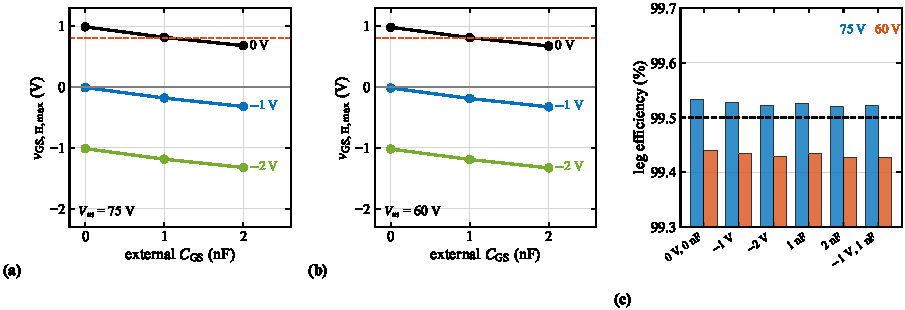
\includegraphics[width=\textwidth]{bump_mitigation.pdf}
\caption{Peak high-side gate voltage against the external gate--source capacitance for off-state biases of 0, $-1$ and $-2$\,V at (a) 75\,V and (b) 60\,V (141\,A); dashed: $V_\mathrm{th,min}$. (c) Leg efficiency at 50\,kHz for the options at 75 and 60\,V.}
\label{fig:mit}
\end{figure}

\begin{table}[t]
\centering\small
\caption{Gate-bump options (141\,A; losses per leg at 50\,kHz, rated point)}
\label{tab:mit}
\setlength{\tabcolsep}{4pt}
\begin{tabular}{@{}clcccccccc@{}}
\toprule
$V_m$ & bias, $C_\mathrm{ext}$ & $v_\mathrm{GS,H,max}$ & $v_\mathrm{GS,H,min}$ & $E_\mathrm{on}$ & $E_\mathrm{off}$ & $P_\mathrm{sw}$ & $P_\mathrm{dead}$ & $P_\mathrm{gate}$ & $\eta$ \\
{[V]} & & [V] & [V] & [\textmu J] & [\textmu J] & [W] & [W] & [W] & [\%] \\
\midrule
\BumpRows
\bottomrule
\end{tabular}
\end{table}

\section{Voltage utilization of the 100\,V transistors}
The submodule voltage $V_m$ determines how well the 100\,V rating is used. At a fixed inverter power and bus voltage the phase current is fixed (100\,A$_\mathrm{rms}$), so the power per leg, and per transistor, is proportional to $V_m$, whereas the conduction and copper losses per leg are not. A higher $V_m$ therefore gives fewer submodules and transistors and a higher efficiency (Fig.~\ref{fig:util}b, c; Table~\ref{tab:util}). The upper limit is the peak drain--source voltage:
\begin{equation}
\hat v_\mathrm{DS}=k\,V_m+\Delta v_\mathrm{os},\qquad k=V_{m,\max}/V_m ,
\end{equation}
where $k$ covers the battery-voltage range and the unbalance of the submodules, and the overshoot is $\Delta v_\mathrm{os}\approx\OvsSF$\,V at 141\,A (\OvsSix\,V at 60\,V; Q3D parasitics, larger at 160\,A). For the original assumption of 75\,V nominal and 90\,V maximum ($k$\,=\,1.2), the peak is \VpkSFk\,V, i.e., above the rating (Fig.~\ref{fig:util}a). Keeping the peak at or below 80\,V, the derating that EPC applies to its own board, allows
\[
V_m\le\VmEighty\,\mathrm{V}\ (k=1.2),\qquad V_m\le\VmEightyK\,\mathrm{V}\ (k=1.0),
\]
and a 90\,V limit allows \VmNinety{} and \VmNinetyK\,V. A nominal submodule voltage of \textbf{60\,V} ($N$\,=\,20 for 1200\,V) gives a peak of \VpkSixk\,V even at $k$\,=\,1.2 and is the recommended design point; 75\,V is only acceptable with a tightly regulated submodule voltage ($k\approx1.0$, peak \VpkSFone\,V). The price of 60\,V is 0.09\,\% inverter efficiency (\EtaSix{} instead of \EtaSF\,\%, \InvLossSix{} instead of \InvLossSF\,W at 150\,kW) and 25\,\% more transistors and drivers; the gate bump is the same at both voltages.

\begin{figure}[t]
\centering
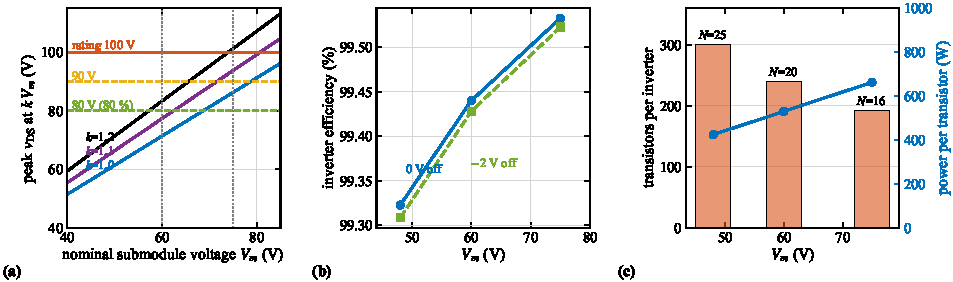
\includegraphics[width=\textwidth]{utilization.pdf}
\caption{Voltage utilization. (a) Peak drain--source voltage against the nominal submodule voltage for maximum-to-nominal ratios $k$\,=\,1.0, 1.1, 1.2 (overshoot from the 141\,A simulations); lines: rating, 90\,V and 80\,V (80\,\% derating). (b) Inverter efficiency at the rated point without and with $-2$\,V off-state bias. (c) Number of transistors of the 1200\,V, 150\,kW inverter and power per transistor ($M$\,=\,1.15).}
\label{fig:util}
\end{figure}

\begin{table}[h]
\centering\small
\caption{Submodule voltage options for the 1200\,V, 150\,kW SPB (two EPC2361 per switch, 50\,kHz)}
\label{tab:util}
\begin{tabular}{@{}lccc@{}}
\toprule
$V_m$ (nominal) & 48\,V & 60\,V & 75\,V \\
\midrule
Submodules $N$ / transistors / drivers & \NsmFE{} / \NtrFE{} / \NdrvFE & \NsmSix{} / \NtrSix{} / \NdrvSix & \NsmSF{} / \NtrSF{} / \NdrvSF \\
Peak $v_\mathrm{DS}$, $k$\,=\,1.0 / 1.2 & \VpkFEone{} / \VpkFEk\,V & \VpkSixone{} / \VpkSixk\,V & \VpkSFone{} / \VpkSFk\,V \\
Voltage utilization $V_m/V_\mathrm{rated}$ & 48\,\% & 60\,\% & 75\,\% \\
Power per transistor ($M$\,=\,1.15) & \PtrFE\,W & \PtrSix\,W & \PtrSF\,W \\
Switching loss per leg & \PswFE\,W & \PswSix\,W & 1.91\,W \\
Inverter efficiency / loss & \EtaFE\,\% / \InvLossFE\,W & \EtaSix\,\% / \InvLossSix\,W & \EtaSF\,\% / \InvLossSF\,W \\
High-side gate bump (0\,V off) & \BmpFortyEight\,V & \BmpSixty\,V & \BmpSeventyFive\,V \\
\bottomrule
\end{tabular}
\end{table}

\section{Recommendations}
\begin{enumerate}
\item Do not reduce the current to fix the bump; it has no effect.
\item Provide a $-1$\,V off-state bias for both gate drives (bipolar auxiliary supply, or a capacitor--Zener level shifter at the driver outputs; check the LT8418 supply limits), or at least place footprints for it, together with do-not-populate gate--source capacitor pads at every gate, so that the measured bump can be corrected on the prototype.
\item Re-evaluate the submodule voltage: with an overshoot of about 11\,V, 75\,V nominal leaves no margin at the maximum battery voltage. Choose $V_m\approx60$\,V ($N$\,=\,20) unless the submodule voltage is regulated tightly, and repeat the overshoot check at 160\,A.
\item Verify on hardware with a double-pulse test and a differential probe on the high-side gate (as on the EPC90156), at room and at operating temperature.
\end{enumerate}

\noindent\small Files: \texttt{simulation/bb\_spice/BB\_bump.cir, BB\_bump\_vth.cir, BB\_bump.inc}; \texttt{scripts/gate\_bump\_study.py}; EPC90156 guide and schematic in \texttt{Datasheet/}.
\end{document}
